\documentclass{article}

\usepackage{amsmath}
\usepackage{amssymb}
\usepackage{graphicx}
\usepackage[german, english]{babel}
\usepackage{caption}


% For at få faver på texten skal man gå til ''Format" og så "Syntax Colering''.
% Her kom jeg til https://www.youtube.com/watch?v=Xl1c_1yL47k

\begin{document}

	\title{Assignment 38}
	\author{pebj, smot}
	\maketitle
		\pagebreak{}

\section{Analysis Object Model (Static Model), including}
\subsection{identifying entity, boundary, and control objects}

\hfill \break Tabel 1.1 entity objects next 1.2\\

\begin{tabular}{l c l @{} l}
	\multicolumn{2}{c}{} \\
	\textbf{Entity Object}&\textbf{Attributes \&Associations}&\textbf{Definition}\\
	\hline
	\textbf{Account}&\parbox{.45\textwidth}{
            \begin{itemize}
                \item MaintainUsers
                \item ManageAccount 
                \item AccountLogic
                \item ManageCalendar
                \item Event
                \item name
                \item email
                \item username
                \item password
            \end{itemize} }
&\parbox{.3\textwidth}{
            An account holds the identification and personal information about a user. } \\
	\hline
	\textbf{Event}&\parbox{.45\textwidth}{
            \begin{itemize}
                \item Account
                \item Alert 
                \item ManageEvent
                \item Description
                \item Date
            \end{itemize} }
&\parbox{.3\textwidth}{
            The event entity describes an event in a calendar. } \\
	\hline
	\textbf{Alert}&\parbox{.45\textwidth}{
            \begin{itemize}
                \item Event
                \item alertionDate
                \item hasBeenSent
            \end{itemize} }
&\parbox{.3\textwidth}{
            An alert holds the information for when a user should be notified about an specific event.  } \\
	\hline
\end{tabular}



		\pagebreak{}

\hfill \break Tabel 1.2 control objects next 1.3\\
\begin{tabular}{l c l @{} l}
	\multicolumn{2}{c}{} \\
	\textbf{Control Object}&\textbf{Attributes \&Associations}&\textbf{Definition}\\
	\hline
	\textbf{Login}&\parbox{.45\textwidth}{
            \begin{itemize}
                \item LoginView
                \item AccountLogic 
            \end{itemize} }
&\parbox{.3\textwidth}{
            The login control object handles login and creation of an account requested from LoginView, these actions will be performed by the related AccountLogic. } \\
	\hline
	\textbf{Server}&\parbox{.45\textwidth}{
            \begin{itemize}
                \item Event
            \end{itemize} }
&\parbox{.3\textwidth}{
            The server is a static online accessable control (webservice etc.) that runs endlessly and regurally checks and sends out alerts to users about upcomming events. } \\
	\hline
	\textbf{ManageCalendar}&\parbox{.45\textwidth}{
            \begin{itemize}
                \item Account
                \item EventLogic
                \item Calendar
            \end{itemize} }
&\parbox{.3\textwidth}{
           ManageCalendar handles all actions done inside Calendar boundary. Any action that would involve an event change/retrival will be done though EventLogic  } \\
	\hline
	\textbf{ManageAccount}&\parbox{.45\textwidth}{
            \begin{itemize}
                \item Account
                \item ManageAccountView
            \end{itemize} }
&\parbox{.3\textwidth}{
            ManageAccount handles all actions done inside ManageAccountView Boundary. Actions that accesses or changes an account will be done though AccountLogic.  } \\



\end{tabular}
	\pagebreak{}

\begin{tabular}{l c l @{} l}
	\multicolumn{2}{c}{} \\
	\hline
	
\textbf{EventLogic}&\parbox{.45\textwidth}{
            \begin{itemize}
                \item MaintainUsers
                \item ManageCalendar
                \item ManageEvent
            \end{itemize} }
&\parbox{.3\textwidth}{
            EventLogic performs any activity that involves getting and changing event entities.  } \\
	\hline
\textbf{AccountLogic}&\parbox{.45\textwidth}{
            \begin{itemize}
                \item ManageAccountView
                \item Account
            \end{itemize} }
&\parbox{.3\textwidth}{
           AccountLogic performs any activity that involves getting and changing Account entities.   } \\
	\hline
\textbf{MaintainUsers}&\parbox{.45\textwidth}{
            \begin{itemize}
                \item AccountLogic
                \item EventLogic
                \item UserAccounts
                \item UserCalendar
            \end{itemize} }
&\parbox{.3\textwidth}{
           MaintainUsers and its related boundaries are reserved to the moderator. It allows him to access and moderate accounts and their events.  } \\
	\hline
\textbf{ManageEvent}&\parbox{.45\textwidth}{
            \begin{itemize}
                \item ManageEventView
                \item EventLogic
                \item Event
            \end{itemize} }
&\parbox{.3\textwidth}{
          ManageEvent handles activities done inside ManageEventView and uses eventlogic if an event has to be updated/added.  } \\
	\hline
\end{tabular}
		\pagebreak{}
\hfill \break Tabel 1.3 boundary objects\\
\begin{tabular}{l c l @{} l}
	\multicolumn{2}{c}{} \\
	\textbf{Boundary Object}&\textbf{Attributes \&Associations}&\textbf{Definition}\\
	\hline
	\textbf{LoginView}&\parbox{.45\textwidth}{
            \begin{itemize}
                \item Login
            \end{itemize} }
&\parbox{.3\textwidth}{
            The login boundary allows the user a way to log into the system and also, to create a new account. } \\
	\hline
	\textbf{UserAccounts}&\parbox{.45\textwidth}{
            \begin{itemize}
                \item MaintainUsers
            \end{itemize} }
&\parbox{.3\textwidth}{
            MaintainUsers boundary allows a moderator to manage (access,edit,remove) user' accounts } \\
	\hline
	\textbf{UserCalendars}&\parbox{.45\textwidth}{
            \begin{itemize}
                \item Account
                \item EventLogic
                \item Calendar
            \end{itemize} }
&\parbox{.3\textwidth}{
           UserCalendars  boundary allows a moderator to get a view over user' events and manage them. } \\
	\hline
	\textbf{ManageEventView}&\parbox{.45\textwidth}{
            \begin{itemize}
                \item ManageEvent
            \end{itemize} }
&\parbox{.3\textwidth}{
            ManageEventView allows a user and moderator to create and edit events.  } \\
	\hline
\textbf{ManageAccountView}&\parbox{.45\textwidth}{
            \begin{itemize}
                \item MaintainUsers
                \item ManageCalendar
                \item ManageEvent
            \end{itemize} }
&\parbox{.3\textwidth}{
            ManageAccountView allows a user to make changes to the attributes of his account, with the exception of username.  } \\
	\hline

\textbf{Calendar}&\parbox{.45\textwidth}{
            \begin{itemize}
                \item ManageCalendar
            \end{itemize} }
&\parbox{.3\textwidth}{
          Calendar allows a user to view and manage his personal calendar.  } \\
	\hline
		\pagebreak{}

\end{tabular}

		
		\pagebreak{}

\subsection{Class Diagram}
\begin{figure}[!htb]
                \caption{Analysis Object Model (Static Model) - class diagram.}
		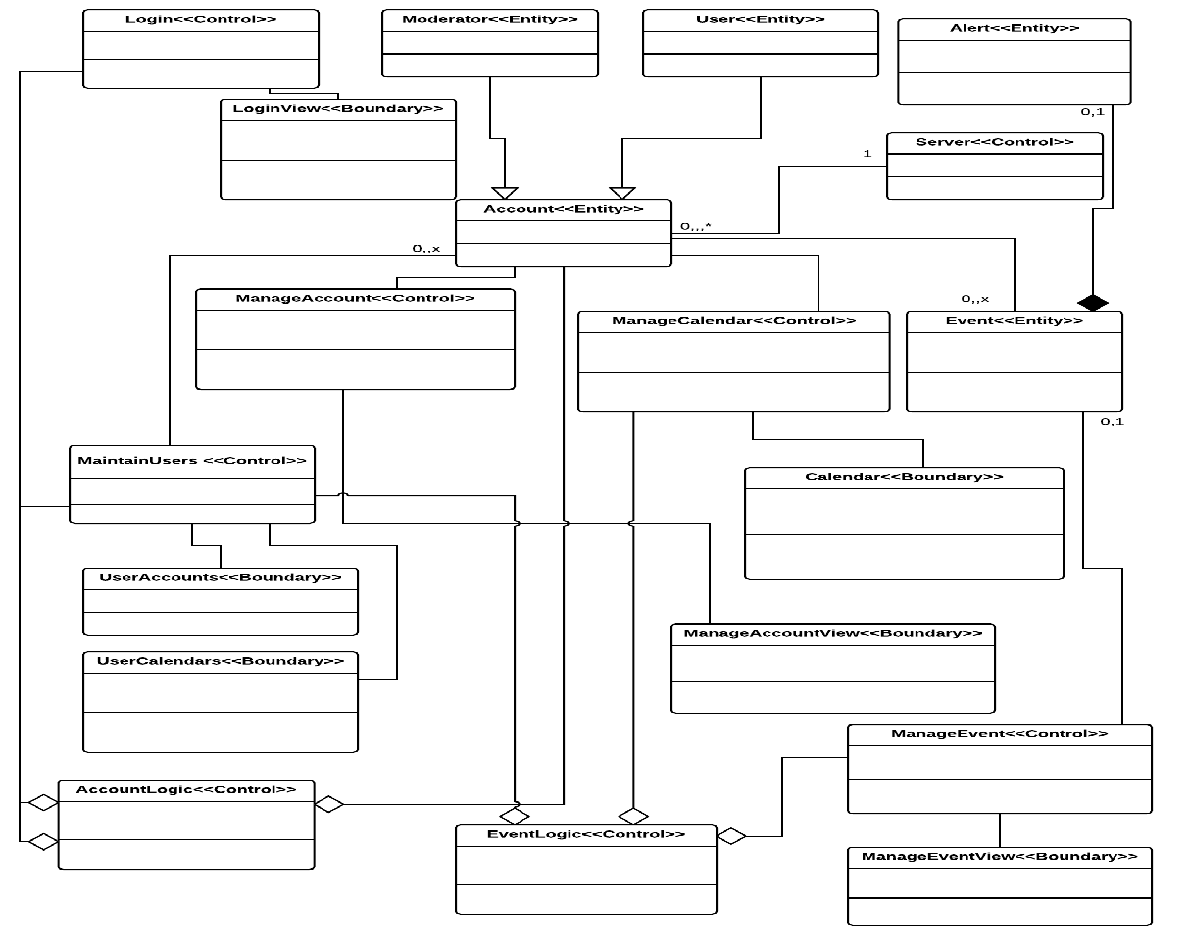
\includegraphics[scale = 0.6]{AnalysisObjectModel.png}\\
		\pagebreak{}
	\end{figure}


		\clearpage

\section{Dynamic Model, including}
\subsection{mapping use cases to sequence Sequence Diagrams involving entity, boundary, and control objects}


	\begin{figure}[!htb]
                \caption{Sequence model for usercase ''Edit personal information''}
		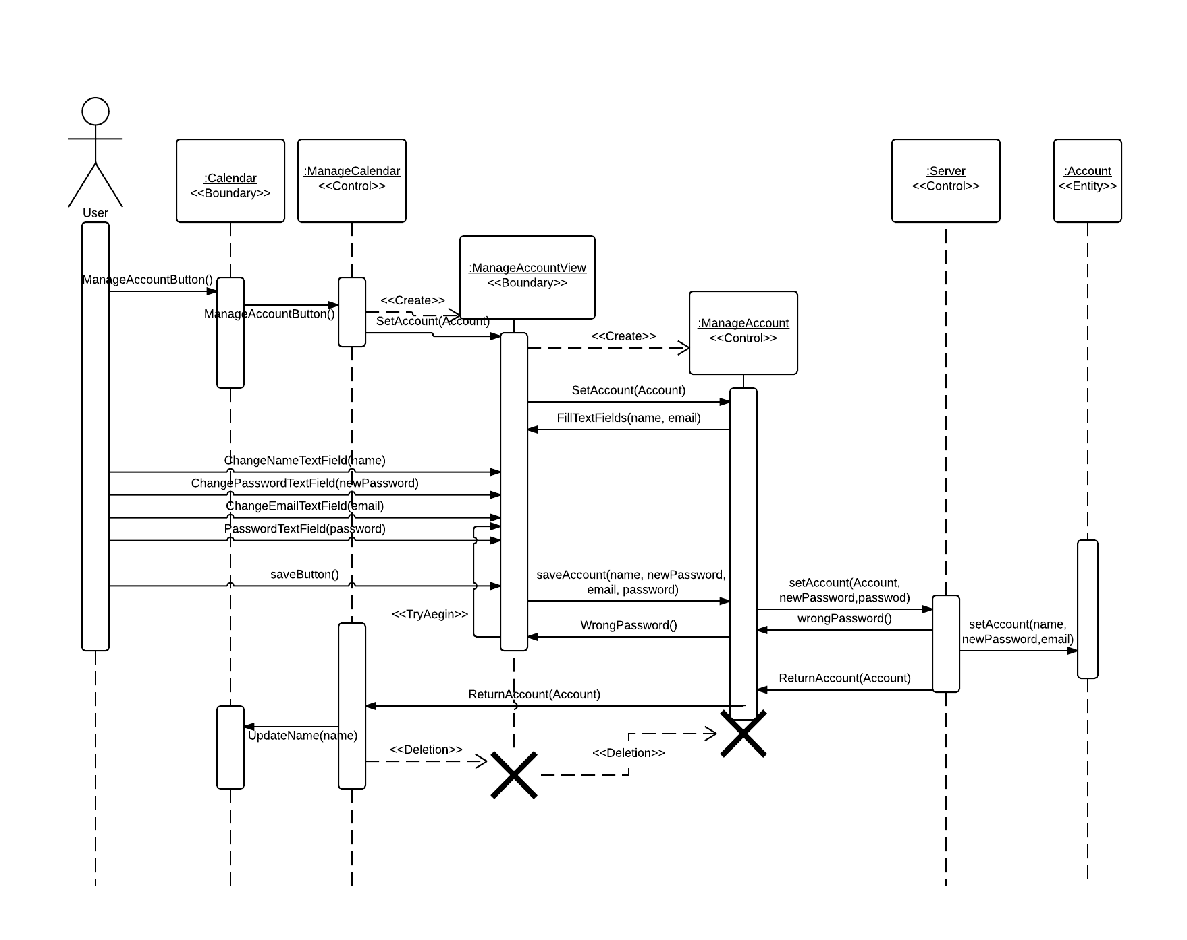
\includegraphics[scale = 0.6]{SequenceModelEditpersonalinformation.png}\\
		\pagebreak{}
	\end{figure}
	
		

	\begin{figure}[!htb]
                \caption{Sequence model for usercase ''enable alert for event''}
		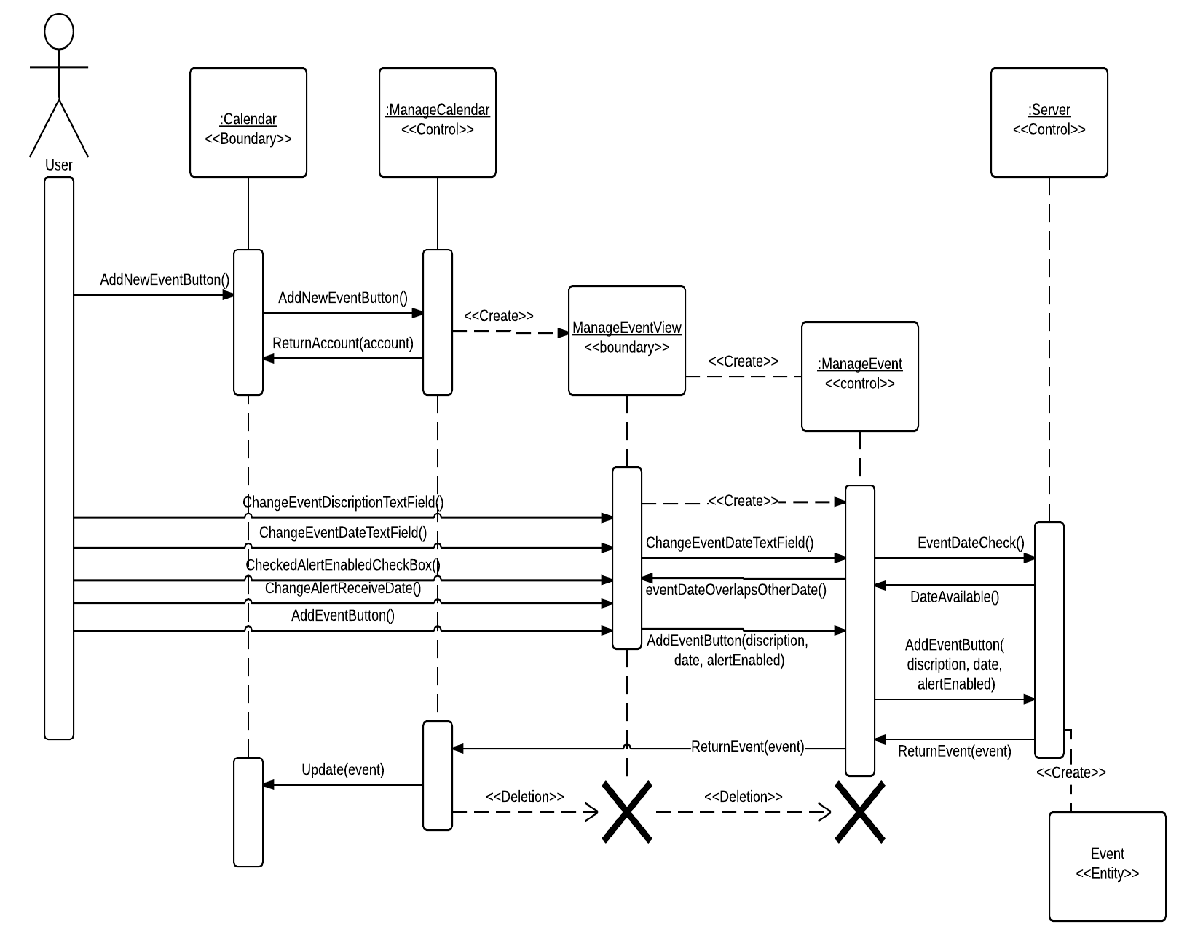
\includegraphics[scale = 0.6]{SequenceModelEnableAlert.png}\\
		\pagebreak{}
	\end{figure}

		\clearpage
	\begin{figure}[!htb]
                \caption{Sequence model for usercase ''Sends a notification (event alert)''}
		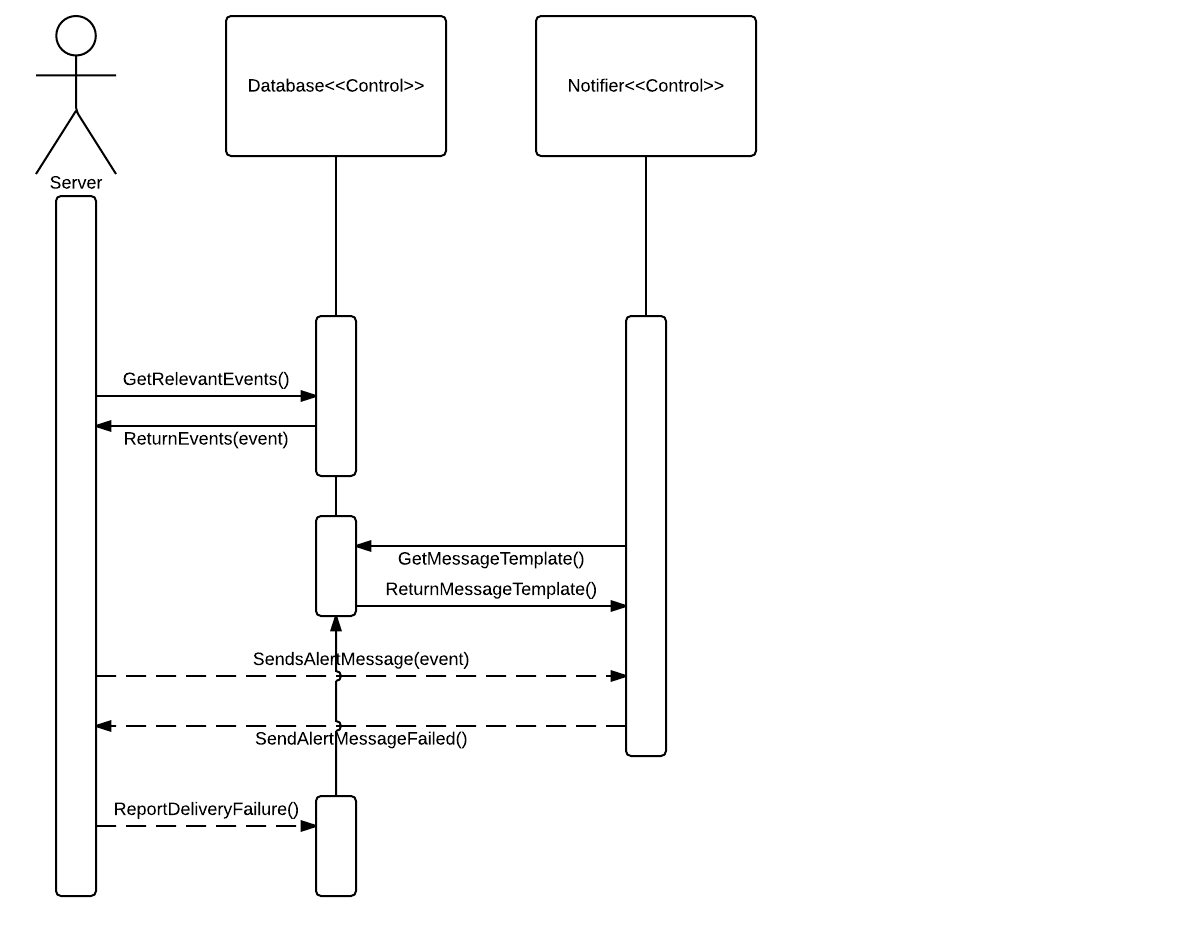
\includegraphics[scale = 0.6]{SequenceModelSendEventAlert.png}\\
		\pagebreak{}
	\end{figure}

		\clearpage
\subsection{modelling state-dependent behavior of individual objects using State Machine Diagrams}


	\begin{figure}[!htb]
                \caption{State Machine Diagram for ''Send alert''}
		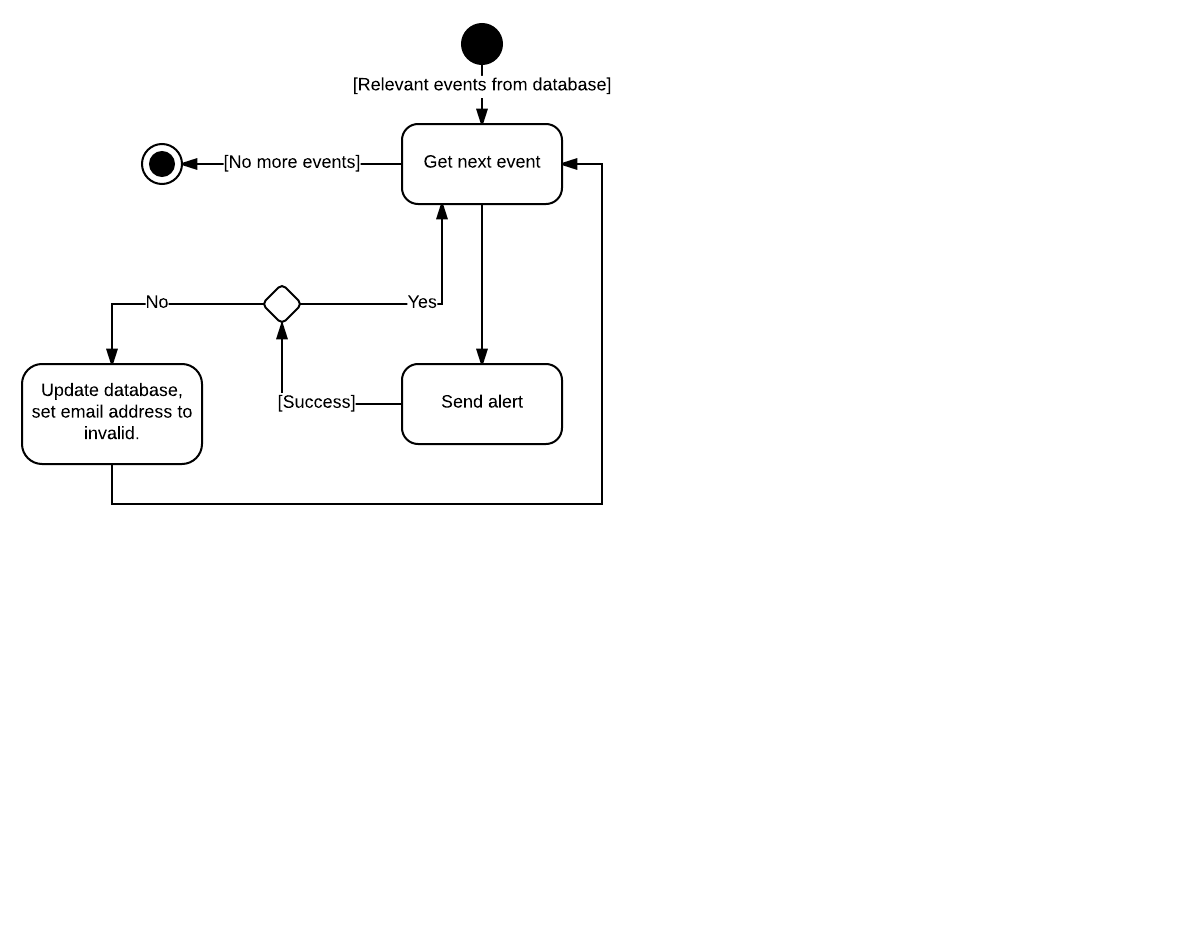
\includegraphics[scale = 0.6]{SendAlertStateMachine.png}\\
		\pagebreak{}
	\end{figure}

	\begin{figure}[!htb]
                \caption{State Machine Diagram for ''New event''}
		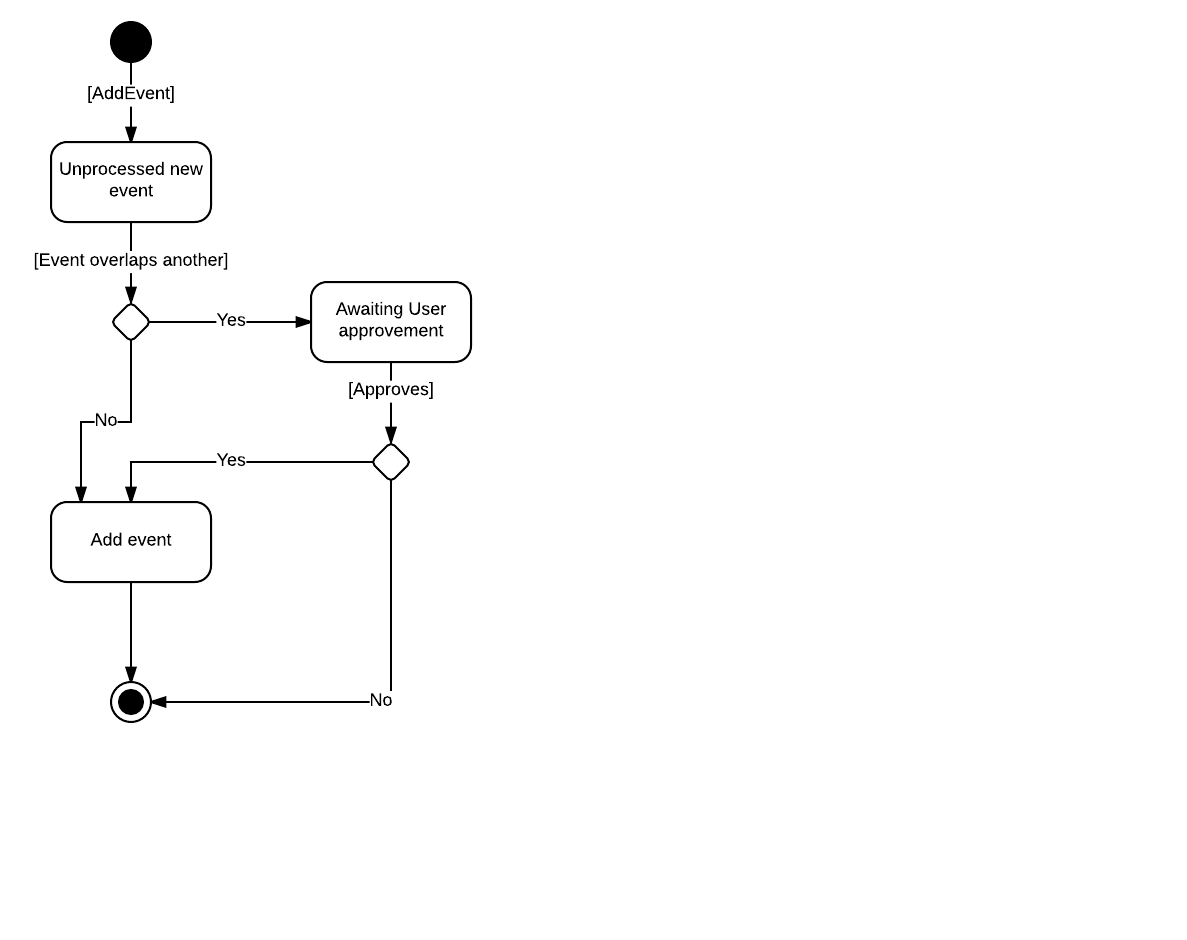
\includegraphics[scale = 0.6]{NewEventStateMachine}\\
		\pagebreak{}
	\end{figure}

\end{document}